\documentclass[a4paper,12pt,twocolumn]{article}
\usepackage[utf8]{inputenc}
\usepackage{graphicx}
\usepackage{hyperref}           % provides automatic hyperlinks to sections and citations automatically
\usepackage[toc,page]{appendix} % allows for an appendix section
\usepackage[cc]{titlepic}       % allows a pic to be included in the title page
\usepackage[table,xcdraw]{xcolor}
\usepackage{comment}            % allows for blocks of comments
\usepackage[normalem]{ulem}     % used for table in table.tex
\useunder{\uline}{\ul}{}        % used for table in table.tex

\title{
    The Effect of Following Distance on an Environment Exploring Rover\\
    \begin{large}
        CM30229 ICCS - Coursework 1 Report
    \end{large}
}
\titlepic{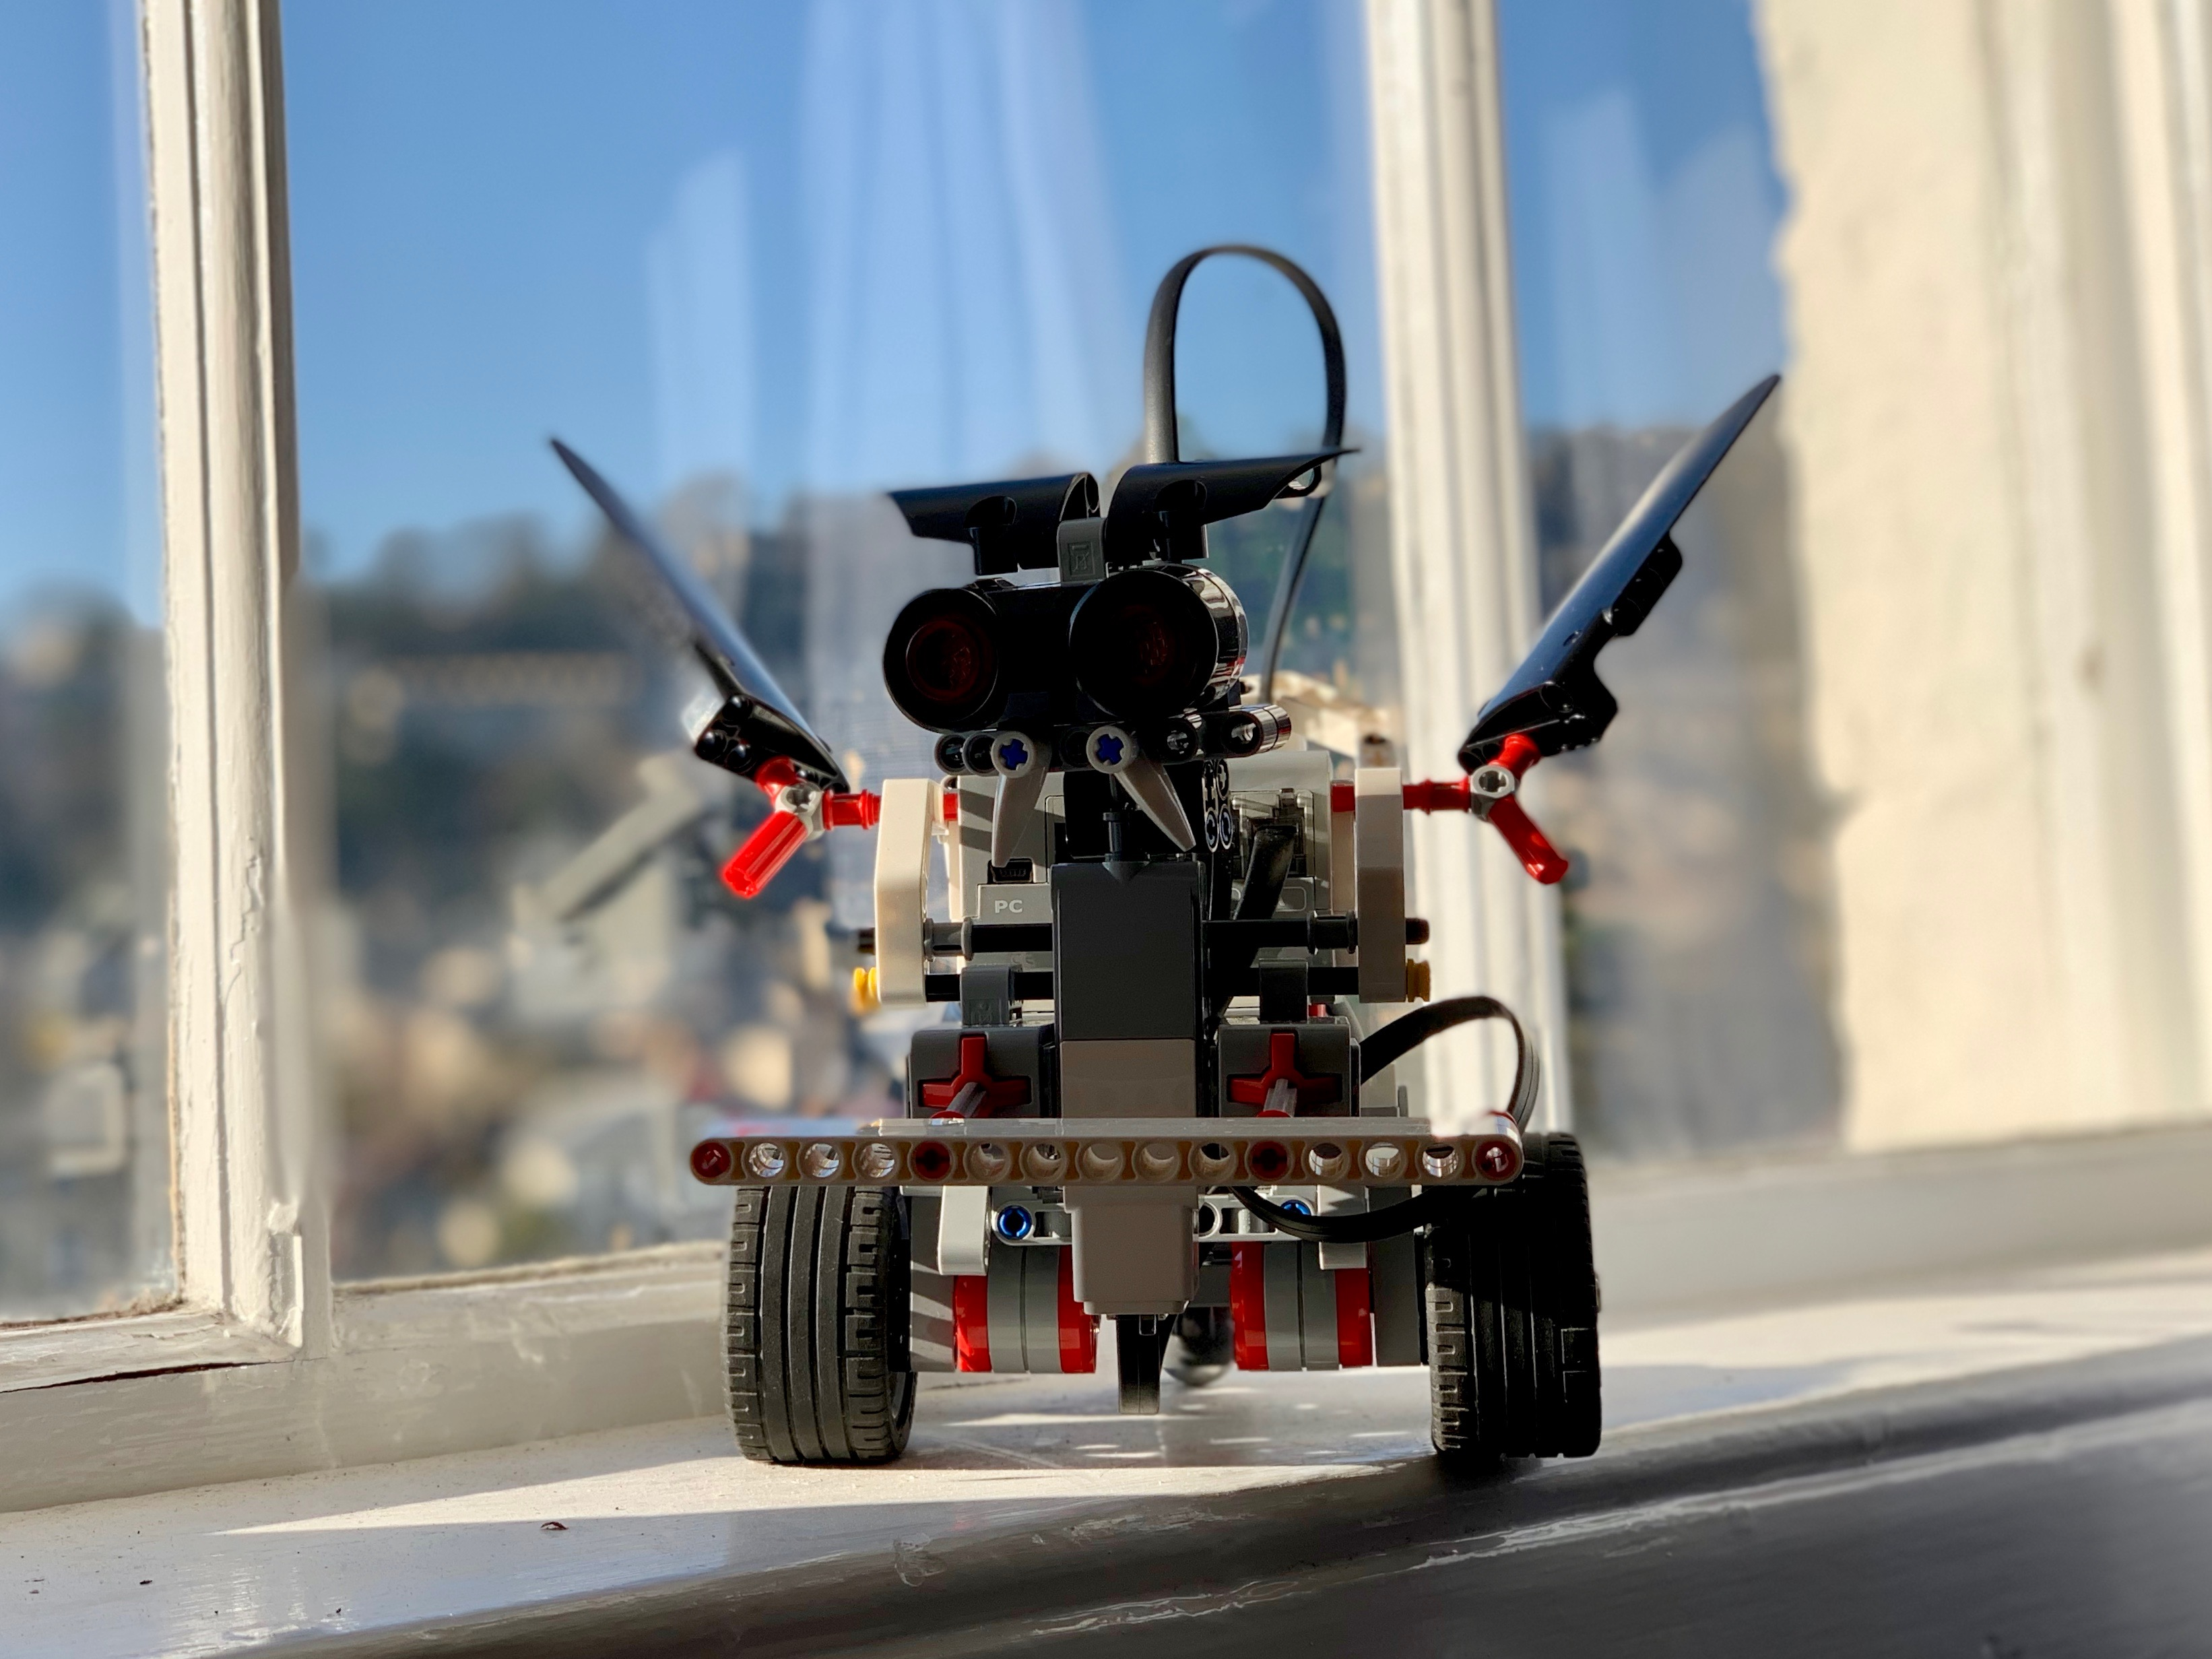
\includegraphics[width=0.90\linewidth]{figures/robot_portrait.jpeg}}
\author{Adam Jaamour & Tom Slattery}
\date{28th February 2019}

\begin{document}
\maketitle
\thispagestyle{empty}
\clearpage
\setcounter{page}{1}

% ----------------------------------------------------------------------------
% ----------------------------------------------------------------------------
% ----------------------------------------------------------------------------

\section{Introduction}

The goal of this research is to determine the effect of changing the wall following distance of a Lego EV3 rover on the number of times it collides with the edges of an arena. This experiment proves the hypothesis that a greater wall following distance results in fewer collisions. The wall following distance is related to both the time taken to traverse a given area and the number of collisions with the walls. It also directly affects the level of granularity with which the rover explores the more detailed parts of the enclosed area. Therefore an optimal traversal of the arena requires the most appropriate following distance to be found. The rover uses a combination of sensors and motors to navigate its environment. It is placed in an arena, consisting of fully enclosing walls.\\

The inspiration for the rover's initial design was the reactive subsumption architecture, with the system consisting of asynchronously communicating parallel layers, each responsible for sub tasks of the wall following algorithm \cite{brooks1991intelligence}. However, subsequent experiment lead to an improved design being based on a simple reflex agent, an architecture which is implemented in series. The rover makes observations in real time and immediately acts on them. Wall following becomes an emergent property of the interactions between preset states of the environment and corresponding actions \cite{wooldridge2009introduction}. While implementing wall following, the rover was altered to store a "wall hit" state while finding the correct direction to turn. As a result, the final rover system is a model based reflex agent \cite{russell1995artificial}. This design proved sufficient to traverse the arena and test the hypothesis.

\section{Approach}
Two types of sensors are used to allow the rover to collect data describing the environment. A pair of touch sensors are mounted on the front of the rover. A bar connects the two sensors for rigidity, allowing angular collisions with corners to be detected. An ultrasonic sensor is mounted on a rotating servo motor at the front of the rover. The high noise floor of the sensor is compensated for by averaging the readings and removing any which are outside of a range of the standard deviation from the mean. The motors were adjusted to compensate for tyre friction by turning more than the desired angle, allowing the rover a more accurate rotation. The rover has "wings" attached on each side of the main body. This was a morphological design decision, preventing the rover from being flipped over by collisions with low objects. The wings can also help to drag the rover around corners.\\

The rover software has three states which can be transitioned between: initial, searching and wall following (Appendix \ref{sec:flowchart}).

The rover begins in the initial state, travelling forwards until a collision is detected. The rover then enters the searching state. The possible configurations of the position of the rover in relation to the arena walls have been simplified to situations observable by the ultrasonic sensor sweeping left and right.
The rover then turns by 90 degrees and rotates the ultrasonic sensor to face the wall. 
To ensure that the rover makes a full clockwise circuit of the arena, it always makes a right turn if possible.
Finally, the rover enters the wall following state and begins moving parallel to the wall. The ultrasonic sensor is used to maintain a constant distance. The rover continues in this state until the touch sensors are triggered again.\\

An arena has been created with enclosing walls, using a variety of concave and convex corners to provide a challenging path for the rover to traverse (Appendix \ref{sec:arena-layout}). The shape of the arena is preserved between trials. A single trial consists of one full lap of the arena. The distance maintained from the wall is an independent variable. The time taken to traverse back to the starting point and the number of wall collisions are dependent variables which are recorded. Two trials are performed for each distance. If the rover becomes stuck or pushes a wall the trial is aborted. The battery charge is kept consistent.



\section{Results}
One main hypothesis was tested by this experiment: maintaining a greater distance during the wall following state results in fewer collisions during a circuit.
The data collected from the experiment is consistent with this hypothesis (Appendix \ref{sec:raw-results}). Increasing distance from the wall results in a downward trend in collisions and shorter lap times (Appendix \ref{sec:graph-results}). A strong correlation between number of collisions and the length of time taken to complete a lap can be seen. It was also observed from visual comparisons of video footage that for larger distances, the rover completely avoided the first book pile, verifying that such distances result in lower detail traversals of the arena (2:39 in the video, Appendix \ref{sec:video-experiment}). 

\begin{comment}
Todo:
\begin{itemize}
    \item state that results are in line with the hypothesis
    \item place results in table
    \item provide link to youtube video
\end{itemize}
\end{comment}

% ----------------------------------------------------------------------------
% ----------------------------------------------------------------------------
% ----------------------------------------------------------------------------

\section{Discussion}
This experiment demonstrated that maintaining a greater distance from the arena walls resulted in fewer collisions. This is particularly important as the searching state entered on collision contributes the longest time spent immobile. The number of collisions is clearly linked to the length of time taken to complete a circuit.\\

Shorter following distances made the rover susceptible to repeated collisions with flat surfaces due to the fixed turning amount while in the wall following state (4:03 in the video, Appendix \ref{sec:video-experiment}). This resulted in many more collisions than necessary, and greatly increased the traversal time. To rectify this, the turning angle could be made proportional to the distance from the wall.

\begin{comment}
Todo:
\begin{itemize}
    \item suggest improvements (more sensors?)
    \item make arena as consistent as possible (obstacles, wall placement, lighting)
\end{itemize}
\end{comment}

% ----------------------------------------------------------------------------
% ----------------------------------------------------------------------------
% ----------------------------------------------------------------------------

\section{Conclusion}

\begin{comment}
Todo:
\begin{itemize}
    \item single paragraph
    \item what this research set out to do and the results of the research
\end{itemize}
\end{comment}

It is shown that a rover which follows walls at a greater distance completes a circuit of an arena with less collisions. It was also observed that a larger distance resulted in a less detailed exploration of the arena. The wall following distance is therefore an important variable which governs the trade-off between speed and accuracy of a traversal.


% ----------------------------------------------------------------------------
% ----------------------------------------------------------------------------
% ----------------------------------------------------------------------------

\onecolumn
\begin{appendices}

\section{Arena Layout}
\label{sec:arena-layout}
\begin{figure}[ht]
\centering
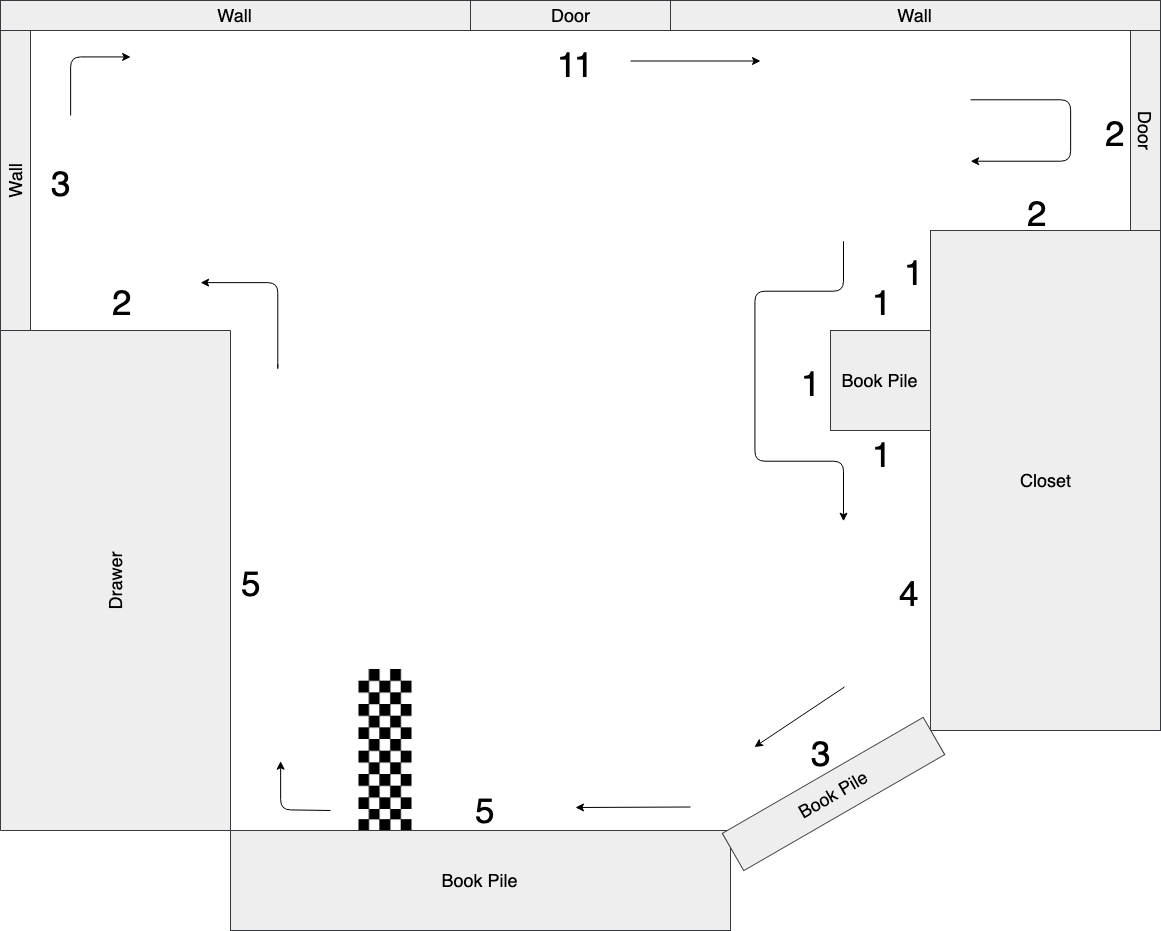
\includegraphics[width=0.60\textwidth]{figures/arena-layout/Arena-Layout.png}
\end{figure}

\section{Flowchart Diagram}
\label{sec:flowchart}
Flowchart diagram describing the rover's three different states and how it transitions between them.
\begin{figure}[ht]
\centerline{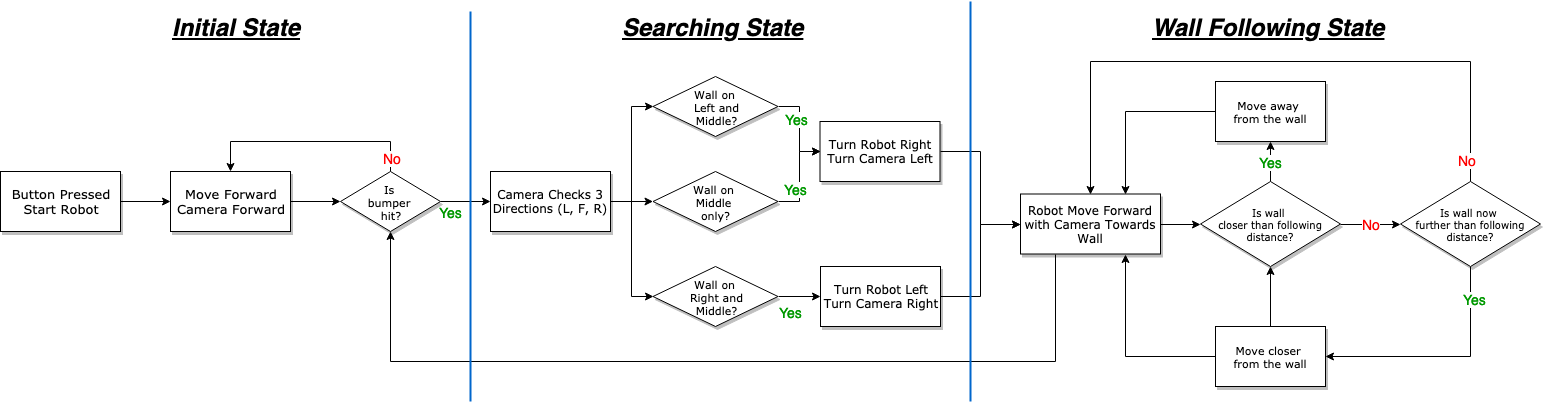
\includegraphics[width=1.25\textwidth]{figures/flowchart/System-Flowchart.png}}
\end{figure}

\section{Video of Experiment}
\label{sec:video-experiment}
A video showcasing the results of the experiment can be found at the following URL: \url{https://www.youtube.com/watch?v=VHsgZ4Ex2-c}.

\section{Graph Results}
\label{sec:graph-results}
Graph showing inverse relation between number of collisions (bumps) and the following distance maintained from the wall. The same relation is shown for time taken for a lap.
\begin{figure}[ht]
\centering
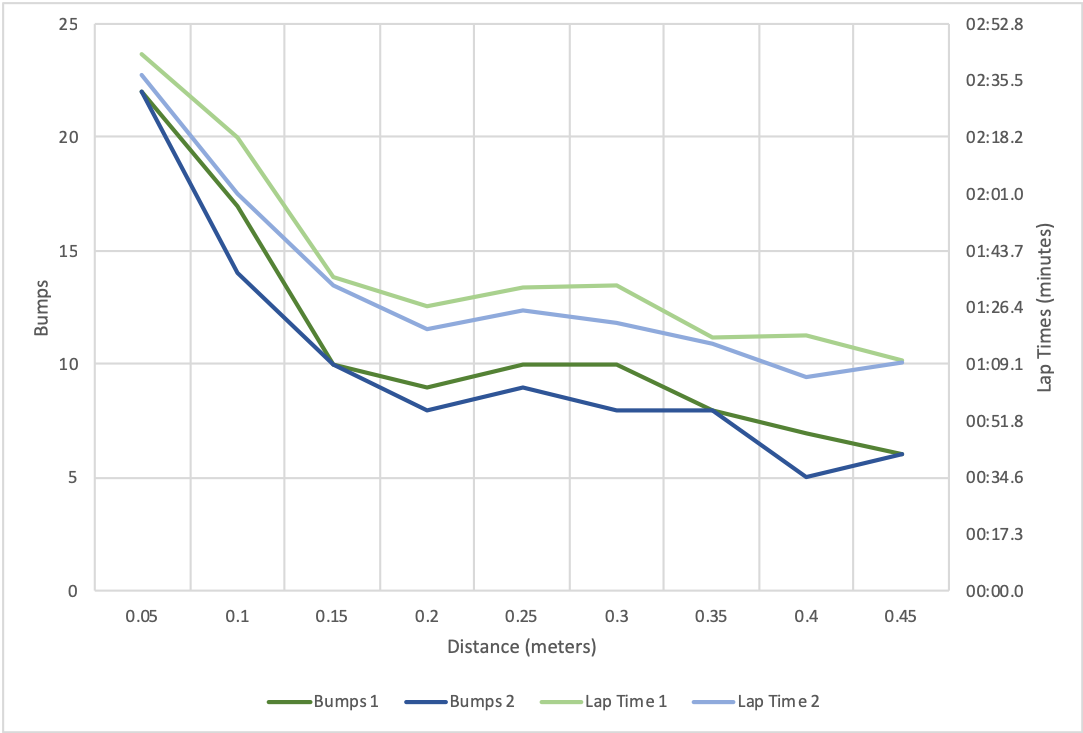
\includegraphics[width=0.65\linewidth]{figures/results_graph.png}
\end{figure}

\section{Raw Results}
\label{sec:raw-results}
\begin{table}[ht]
\begin{tabular}{l|l|l|l|l|}
\cline{2-5}
                                        & \multicolumn{2}{c|}{\textbf{Trial 1}}                & \multicolumn{2}{c|}{\textbf{Trial 2}}                \\ \hline
\multicolumn{1}{|l|}{\textbf{Distance}} & \textit{\textbf{Bumps}} & \textit{\textbf{Lap Time}} & \textit{\textbf{Bumps}} & \textit{\textbf{Lap Time}} \\ \hline
\multicolumn{1}{|l|}{\textbf{0.05}}     & 22                      & 02:43.8                    & 22                      & 02:37.0                    \\ \hline
\multicolumn{1}{|l|}{\textbf{0.1}}      & 17                      & 02:18.0                    & 14                      & 02:01.0                    \\ \hline
\multicolumn{1}{|l|}{\textbf{0.15}}     & 10                      & 01:35.7                    & 10                      & 01:33.3                    \\ \hline
\multicolumn{1}{|l|}{\textbf{0.2}}      & 9                       & 01:26.6                    & 8                       & 01:19.6                    \\ \hline
\multicolumn{1}{|l|}{\textbf{0.25}}     & 10                      & 01:32.0                    & 9                       & 01:25.0                    \\ \hline
\multicolumn{1}{|l|}{\textbf{0.3}}      & 10                      & 01:33.3                    & 8                       & 01:22.0                    \\ \hline
\multicolumn{1}{|l|}{\textbf{0.35}}     & 8                       & 01:17.5                    & 8                       & 01:15.6                    \\ \hline
\multicolumn{1}{|l|}{\textbf{0.4}}      & 7                       & 01:17.8                    & 5                       & 01:05.0                    \\ \hline
\multicolumn{1}{|l|}{\textbf{0.45}}     & 6                       & 01:10.3                    & 6                       & 01:09.9                    \\ \hline
\end{tabular}
\end{table}
\end{appendices}

% ----------------------------------------------------------------------------
% ----------------------------------------------------------------------------
% ----------------------------------------------------------------------------

\clearpage
\bibliographystyle{apalike}
\bibliography{bibliography}

\end{document}